\documentclass[border=6pt]{standalone}
\usepackage{tikz}
\usetikzlibrary{arrows.meta,positioning,calc,shapes.geometric,fit,backgrounds,patterns,matrix,decorations.pathreplacing}
\begin{document}
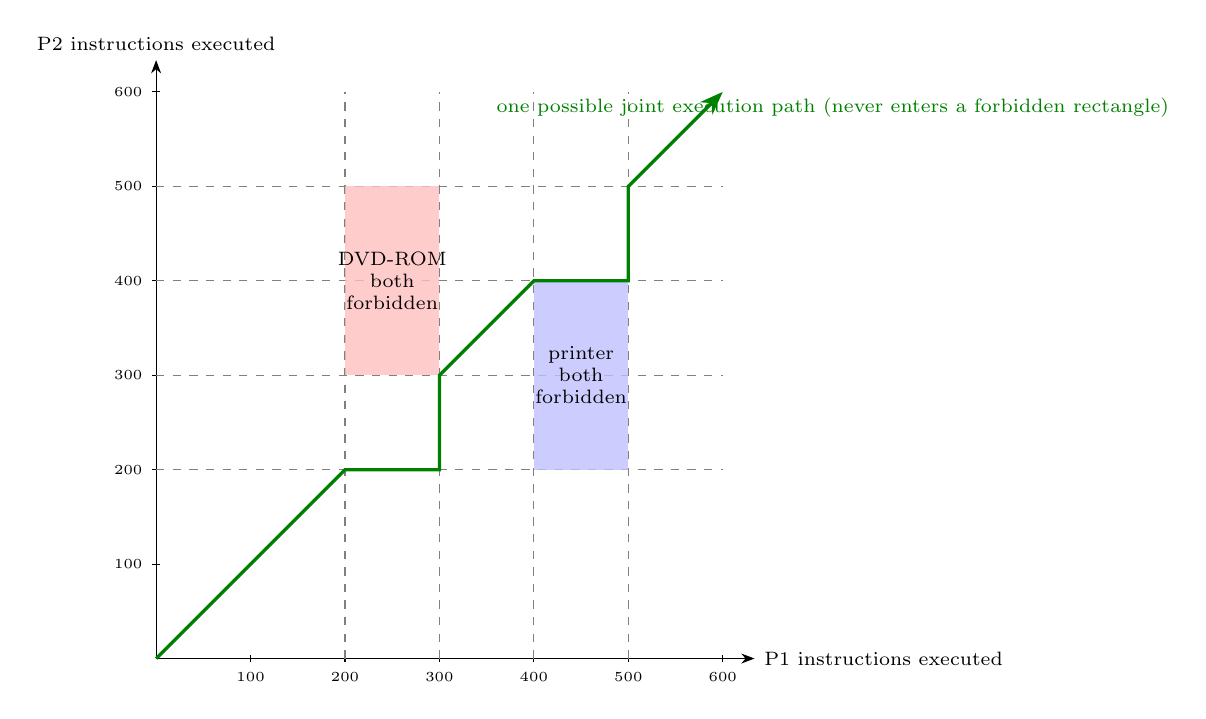
\begin{tikzpicture}[>=Stealth,font=\small]
\def\s{0.012}
\draw[->] (0,0) -- (7.6,0) node[right,font=\scriptsize]{P1 instructions executed};
\draw[->] (0,0) -- (0,7.6) node[above,font=\scriptsize]{P2 instructions executed};
\foreach \v in {100,200,300,400,500,600} { \draw (\v*\s,0.05) -- (\v*\s,-0.05) node[below,font=\tiny]{\v}; \draw (0.05,\v*\s) -- (-0.05,\v*\s) node[left,font=\tiny]{\v}; }
\draw[dashed,gray] (200*\s,0) -- (200*\s,7.2); \draw[dashed,gray] (300*\s,0) -- (300*\s,7.2);
\draw[dashed,gray] (400*\s,0) -- (400*\s,7.2); \draw[dashed,gray] (500*\s,0) -- (500*\s,7.2);
\draw[dashed,gray] (0,200*\s) -- (7.2,200*\s); \draw[dashed,gray] (0,300*\s) -- (7.2,300*\s); \draw[dashed,gray] (0,400*\s) -- (7.2,400*\s); \draw[dashed,gray] (0,500*\s) -- (7.2,500*\s);
\fill[red!25,opacity=0.8] (200*\s,300*\s) rectangle (300*\s,500*\s);
\fill[blue!25,opacity=0.8] (400*\s,200*\s) rectangle (500*\s,400*\s);
\node[font=\scriptsize,align=center] at (250*\s,400*\s) {DVD-ROM\\ both\\ forbidden};
\node[font=\scriptsize,align=center] at (450*\s,300*\s) {printer\\ both\\ forbidden};
\draw[very thick,green!50!black,->] (0,0) -- (200*\s,200*\s) -- (300*\s,200*\s) -- (300*\s,300*\s) -- (400*\s,400*\s) -- (500*\s,400*\s)--(500*\s,500*\s) -- (600*\s,600*\s);
\node[font=\scriptsize,green!50!black,anchor=west] at (4.2,7.0) {one possible joint execution path (never enters a forbidden rectangle)};
\end{tikzpicture}
\end{document}
